%	- present toy examples and what they are testing
%		- these should be quite good
%	- refer to UCI datasets as well-known evaluation platforms for regression

In this section, we will empirically evaluate the proposed \acp{RFSF}.
We aim to assess the following central hypothesis:
\begin{enumerate}
    \item Do \acp{RFSF} outperform \acp{RFF} (due to their increased parameter capacity)?
\end{enumerate}
Additionally, we try to answer the following questions:
\begin{enumerate}  \setcounter{enumi}{1}
    \item Does the increased amount of parameters lead to overfitting?
    \item How do different initial values of the features' amplitudes affect the performance?
\end{enumerate}
In the following, we will first present some implementation details (\autoref{subsec:impl}) and subsequently present the experiment setup (\autoref{subsec:setup}) and results (\autoref{subsec:results}).


\subsection{Implementation}  \label{subsec:impl}
We implemented \acp{RFSF} using GPyTorch\cite{jacotNeuralTangentKernel2020} and used Adam\cite{kingmaAdamMethodStochastic2017a} for maximizing the marginal log-likelihood.
Despite the computational advantage of not having to compute (and, most importantly, invert) the Gram matrix, we implemented \acp{RFSF} directly as a GPyTorch kernel.
This allowed a unified view and evaluation when comparing to well-known kernels like the \ac{SE} kernel.
Also, it allowed to just modifying the existing code for \acp{RFF}, reducing the risk of implementation errors.
We published our implementation on \href{https://github.com/fdamken/random-fourier-series-features}{GitHub}\footnote{\url{https://github.com/fdamken/random-fourier-series-features}}.


\subsection{Experiment Setup}  \label{subsec:setup}
To assess our hypothesis, we evaluate our approach on three classes of data sets: synthetic (\autoref{tab:dataSynthetic}), \ac{UCI}\cite{duaUCIMachineLearning2017} (\autoref{tab:dataUci}), and robotics (real data from a cartpole with the states as inputs and control signal as target).
The model quality is measured by the \ac{RMSE} and log-likelihood on the test data (using the test/train splits provided along\cite{galDropoutBayesianApproximation2016} for a fair comparison).
For \ac{RFSF}, we assess three different initializations of the amplitudes:
\begin{itemize}
    \item \emph{Random (Rand.):}       Sampled from a uniform distribution, i.e., $\vec{a}_{0:M}, \vec{b}_{0:M} \sim \mathcal{U}(0, 1)$.
    \item \emph{\ac{ReLU}:}            Taken from the Fourier series for a periodic \ac{ReLU}, i.e., $a_m = (\tilde{T} (-1)^m - \tilde{T}) / (m^2 \pi^2)$ and $b_m = -(\tilde{T} (-1)^m) / (m \pi)$ for $m > 0$ and $a_0 = \tilde{T}/2$ and $b_0 = 0$ (see \autoref{app:perelu} for further details and the derivation).
    \item \emph{Single Harmonic (SH):} All set to zero except for the $0$-th which are set to one, i.e., $a_0 = b_0 = 1$, $\vec{a}_{1:M} = \vec{b}_{1:M} = \vec{0}$.
\end{itemize}
The idea behind each is as follows.
The random initialization is most simplistic and a baseline for the others.
Initializing the amplitudes as (periodic) \acp{ReLU} sets the connection to kernel learning and \acp{BNN} with the \ac{ReLU} being one of the most common activation functions.
Starting with a single harmonic similar to \acp{RFF} connects \acp{RFSF} closer to the idea behind \acp{RFF} and serves as an assessment of our hypothesis that \acp{RFSF} should have higher capacity than \acp{RFF} (i.e., if the marginal log-likelihood would not get better by touching the other amplitudes, they shall not change).

We compare our method to the \ac{SE} and \ac{RFF} kernel.
For some data sets (\ac{UCI} Boston, concrete, power, and yacht), we also compare to popular approaches for \acp{BNN}:
\begin{itemize}
    \item A \ac{BLL} \ac{NN} with Gaussian conjugate prior on the weight. With $\vec{\phi}_{\vec{\theta}}(\vec{x})$ being the parameterized features induced by the \ac{NN} and $\mat{\Lambda}_0$ being the covariance of the prior, this is equivalent to a \ac{GP} with kernel $k_{\vec{\theta}}(\vec{x}, \vec{y}) = \vec{\phi}_{\vec{\theta}}(\vec{x})^\transposed \mat{\Lambda}_0^{-1} \vec{\phi}_{\vec{\theta}}(\vec{y})$\cite{rasmussenGaussianProcessesMachine2006}.
    \item Ensemble  \todo{describe}
    \item MAP  \todo{describe}
\end{itemize}
\todo{STOPPED HERE}

\begin{table}
    \centering
    \begin{tabular}{lll}
        \toprule
        \textbf{Name} & \textbf{Function}         & \textbf{Domain}                   \\ \midrule
        Cosine        & $\cos(2 \pi x)$           & $[-0.5, 0.5]$                     \\
        Heaviside     & $\Theta(x)$               & $[-0.5, 0.5]$                     \\
        Heavi-Cosine  & $\Theta(x) \cos(2 \pi x)$ & $[-0.5, 0.5]$                     \\
        Gap-Cosine    & $\cos(2 \pi x)$           & $[-0.75, -0.25) \cup (0.5, 0.75]$ \\
        \bottomrule
    \end{tabular}
    \caption{Synthetic Data Sets}
    \label{tab:dataSynthetic}
\end{table}

\begin{table}
    \centering
    \begin{tabular}{lll}
        \toprule
        \textbf{Name}                 & \textbf{Short Name} & \textbf{Source}\cite{duaUCIMachineLearning2017}       \\ \midrule
        Boston Housing                & Boston   &                                                                  \\
        Concrete Compression Strength & Concrete & \cite{yehModelingStrengthHighperformance1998}                    \\
        Combined Cycle Power Plant    & Power    & \cite{kayaLocalGlobalLearning2012,tufekciPredictionFullLoad2014} \\
        Yacht                         & Yacht    &                                                                  \\
        Energy Efficiency             & Energy   & \cite{tsanasAccurateQuantitativeEstimation2012}                  \\
        Kinematics of 8-Link Robot    & Kin8nm   &                                                                  \\
        Naval Propulsion Plants       & Naval    & \cite{coradduMachineLearningApproaches2016}                      \\
        Protein Tertiary Structure    & Protein  &                                                                  \\
        Wine Quality (Red)            & Wine     & \cite{cortezModelingWinePreferences2009}                         \\
        \bottomrule
    \end{tabular}
    \caption{\acs{UCI} Data Sets}
    \label{tab:dataUci}
\end{table}


\subsection{Results}  \label{subsec:results}
We first compare visually the quality of \acp{RFSF} to the \ac{RBF} kernel on the synthetic data.
As this data is one-dimensional, it is straightforward to plot it.
\autopageref{fig:syntheticResultPlot} shows the results of the aforementioned kernels on the synthetic data.
For \acp{RFSF}, it can be seen that the mean prediction along with the uncertainty estimation are reasonable and match the true function exactly in vicinity of the training samples.
The same holds for the \ac{RBF} kernel.



\begin{figure*}
    \centering
    \begin{subfigure}{0.49\linewidth}
        \centering
        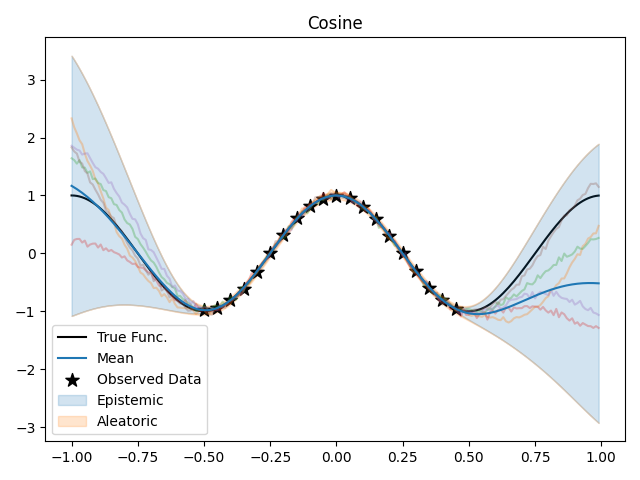
\includegraphics[width=\linewidth, height=0.618033988749895\linewidth]{graphics/generated/gp-cosine-rfsf.png}  % TODO: Replace PNG with TikZ
        \caption{Results of the \acs{RFSF} kernel on the cosine data set.}
    \end{subfigure}
    \begin{subfigure}{0.49\linewidth}
        \centering
        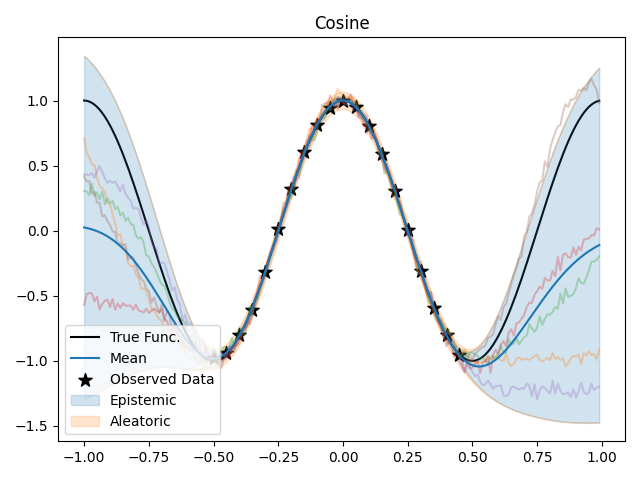
\includegraphics[width=\linewidth, height=0.618033988749895\linewidth]{graphics/generated/gp-cosine-rbf.png}  % TODO: Replace PNG with TikZ
        \caption{Results of the \acs{RBF} kernel on the cosine data set.}
    \end{subfigure}
	\\[0.5cm]
    \begin{subfigure}{0.49\linewidth}
        \centering
        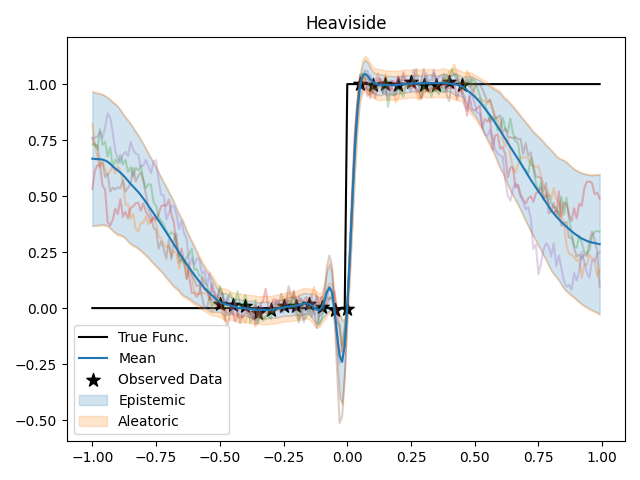
\includegraphics[width=\linewidth, height=0.618033988749895\linewidth]{graphics/generated/gp-heaviside-rfsf.png}  % TODO: Replace PNG with TikZ
        \caption{Results of the \acs{RFSF} kernel on the heaviside data set.}
    \end{subfigure}
	~
    \begin{subfigure}{0.49\linewidth}
        \centering
        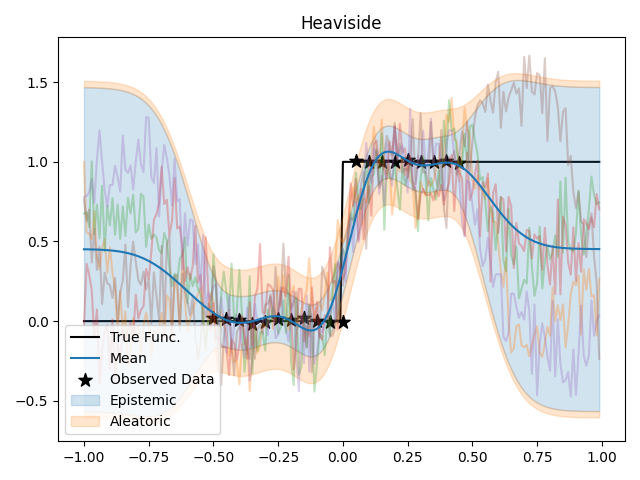
\includegraphics[width=\linewidth, height=0.618033988749895\linewidth]{graphics/generated/gp-heaviside-rbf.png}  % TODO: Replace PNG with TikZ
        \caption{Results of the \acs{RBF} kernel on the heaviside data set.}
    \end{subfigure}
    \\[0.5cm]
    \begin{subfigure}{0.49\linewidth}
        \centering
        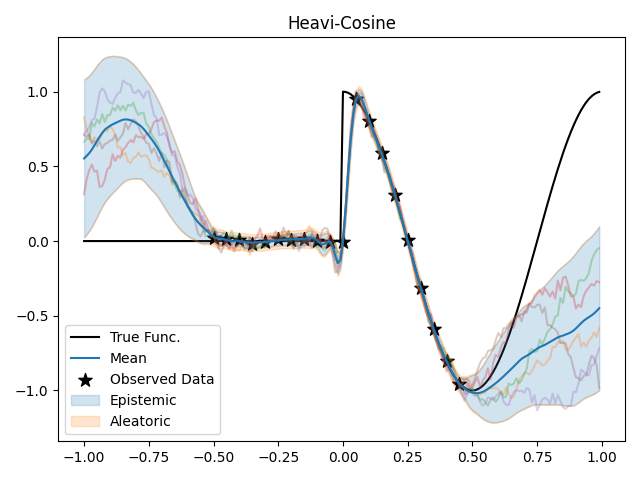
\includegraphics[width=\linewidth, height=0.618033988749895\linewidth]{graphics/generated/gp-heavicosine-rfsf.png}  % TODO: Replace PNG with TikZ
        \caption{Results of the \acs{RFSF} kernel on the heavi-cosine data set.}
    \end{subfigure}
	~
    \begin{subfigure}{0.49\linewidth}
        \centering
        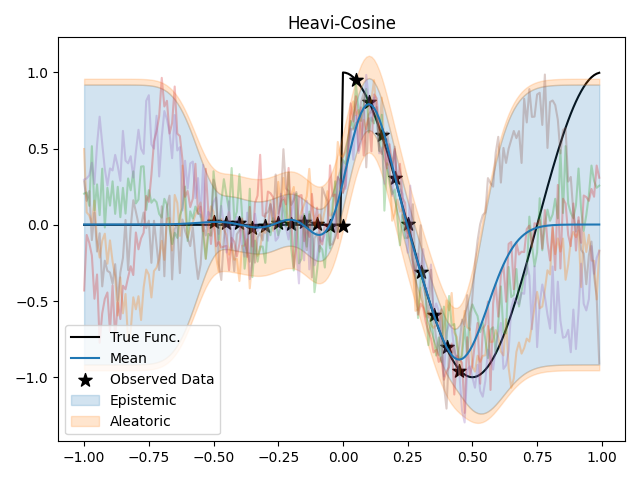
\includegraphics[width=\linewidth, height=0.618033988749895\linewidth]{graphics/generated/gp-heavicosine-rbf.png}  % TODO: Replace PNG with TikZ
        \caption{Results of the \acs{RBF} kernel on the heavi-cosine data set.}
    \end{subfigure}
    \\[0.5cm]
    \begin{subfigure}{0.49\linewidth}
        \centering
        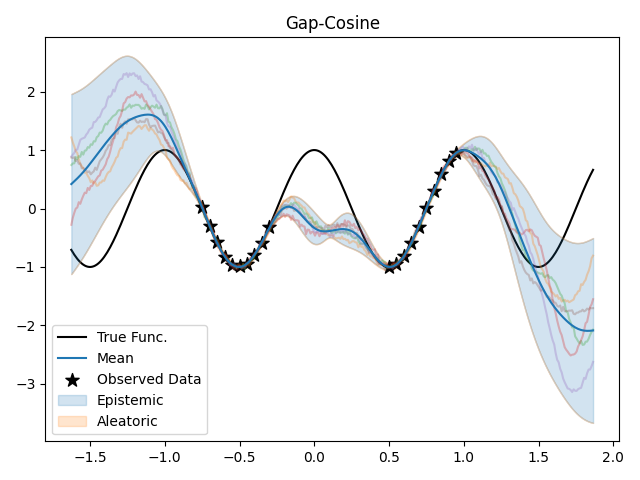
\includegraphics[width=\linewidth, height=0.618033988749895\linewidth]{graphics/generated/gp-gapcosine-rfsf.png}  % TODO: Replace PNG with TikZ
        \caption{Results of the \acs{RFSF} kernel on the gap-cosine data set.}
    \end{subfigure}
	~
    \begin{subfigure}{0.49\linewidth}
        \centering
        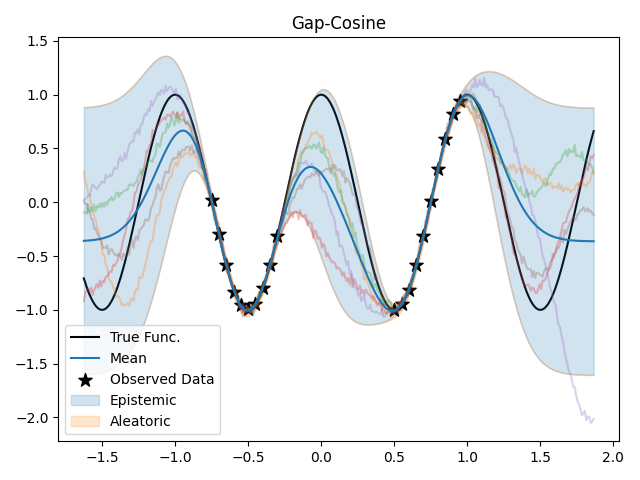
\includegraphics[width=\linewidth, height=0.618033988749895\linewidth]{graphics/generated/gp-gapcosine-rbf.png}  % TODO: Replace PNG with TikZ
        \caption{Results of the \acs{RBF} kernel on the gap-cosine data set.}
    \end{subfigure}
    \caption{
        \acl{GP} regression results using an \acsp{RFSF} kernel for the synthetic data sets.
        The shaded areas depict the epistemic/aleatoric (posterior) uncertainty, the blue solid line depicts the (posterior) mean, the black stars are the training samples, and the black solid line depicts the true function.
        The colorful lines are samples from the \acsp{GP}.
        Axis labels and ticks where left out for brevity as the results are purely qualitative and specific numbers do not matter.
    }
    \label{fig:syntheticResultPlot}
\end{figure*}

\begin{table*}
    \centering
    \begin{subtable}{\linewidth}
        \centering
        \begin{tabular}{c|cc|ccccc}
            \toprule
            & & & \multicolumn{5}{c}{\textbf{Data Set}} \\[1pt]
            & \multicolumn{2}{c|}{\textbf{Model}} & Cosine                 & Heaviside              & Heavi-Cosine            & Gap-Cosine             & Cartpole                          \\
            \midrule \multirow{5}{*}{\rotatebox{90}{\textbf{Log-Lik.}}}
            & \multirow[t]{3}{*}{RFSF} & Rand.    & \textbf{\texttt{2.43}} & \texttt{0.11}          & \texttt{-1.66}          & \texttt{1.27}          & \texttt{~-9.88\,±\,1.86}          \\
            &                          & ReLU     & \texttt{2.34}          & \textbf{\texttt{0.80}} & \texttt{-0.90}          & \texttt{1.50}          & \texttt{-12.30\,±\,2.31}          \\
            &                          & SH       & \texttt{2.37}          & \textbf{\texttt{0.21}} & \texttt{-1.23}          & \texttt{1.52}          & \texttt{~-9.73\,±\,2.10}          \\
            & \multirow[t]{2}{*}{GP}   & RBF      & \textbf{\texttt{2.44}} & \texttt{0.73}          & \textbf{\texttt{~0.77}} & \textbf{\texttt{2.58}} & \textbf{\texttt{~-3.21\,±\,1.64}} \\
            &                          & RFF      & \textbf{\texttt{2.44}} & \texttt{0.73}          & \textbf{\texttt{~0.78}} & \textbf{\texttt{2.59}} & \texttt{~-7.38\,±\,1.94}          \\
            \midrule \multirow{5}{*}{\rotatebox{90}{\textbf{RMSE}}}
            & \multirow[t]{3}{*}{RFSF} & Rand.    & \texttt{0.45}          & \texttt{0.35}          & \texttt{~0.55}          & \texttt{0.91}          & \texttt{~~0.91\,±\,0.08}          \\
            &                          & ReLU     & \textbf{\texttt{0.39}} & \texttt{1.06}          & \texttt{~3.55}          & \texttt{1.62}          & \texttt{~~1.01\,±\,0.10}          \\
            &                          & SH       & \texttt{0.70}          & \texttt{0.35}          & \texttt{~0.48}          & \texttt{0.75}          & \texttt{~~0.98\,±\,0.11}          \\
            & \multirow[t]{2}{*}{GP}   & RBF      & \texttt{0.45}          & \texttt{0.30}          & \textbf{\texttt{~0.29}} & \textbf{\texttt{0.40}} & \textbf{\texttt{~~0.77\,±\,0.07}} \\
            &                          & RFF      & \texttt{0.45}          & \texttt{0.31}          & \textbf{\texttt{~0.30}} & \texttt{0.42}          & \texttt{~~1.26\,±\,0.10}          \\
            \bottomrule
        \end{tabular}
        \caption{Results for the synthetic data sets and cartpole.}
    \end{subtable}
    \\[0.5cm]
    \begin{subtable}{\linewidth}
        \centering
        \begin{tabular}{c|cc|cccc}
            \toprule
            & & & \multicolumn{4}{c}{\textbf{Data Set}} \\[1pt]
            & \multicolumn{2}{c|}{\textbf{Model}}                   & Boston                           & Concrete                         & Power                            & Yacht                            \\
            \midrule \multirow{11}{*}{\rotatebox{90}{\textbf{Log-Lik.}}}
            & \multirow[t]{3}{*}{RFSF}                 & Rand.      & \texttt{-2.40\,±\,0.05}          & \textbf{\texttt{-2.94\,±\,0.05}} & \texttt{-2.78\,±\,0.01}          & \texttt{-0.80\,±\,0.02}          \\
            &                                          & ReLU       & \texttt{-2.39\,±\,0.05}          & \textbf{\texttt{-2.93\,±\,0.04}} & \texttt{-2.80\,±\,0.01}          & \texttt{-0.86\,±\,0.02}          \\
            &                                          & SH         & \texttt{-2.44\,±\,0.06}          & \textbf{\texttt{-2.94\,±\,0.05}} & \texttt{-2.78\,±\,0.01}          & \texttt{-0.83\,±\,0.02}          \\
            & \multirow[t]{2}{*}{GP}                   & RBF        & \textbf{\texttt{-2.38\,±\,0.05}} & \textbf{\texttt{-2.98\,±\,0.06}} & \texttt{-2.82\,±\,0.01}          & \texttt{-0.80\,±\,0.02}          \\
            &                                          & RFF        & \texttt{-2.40\,±\,0.06}          & \textbf{\texttt{-3.01\,±\,0.05}} & \texttt{-2.84\,±\,0.01}          & \texttt{-0.80\,±\,0.02}          \\
            & \multirow[t]{2}{*}{GBLL}\superdagger     & Leaky ReLU & \texttt{-2.90\,±\,0.05}          & \texttt{-3.09\,±\,0.03}          & \texttt{-2.77\,±\,0.01}          & \texttt{-1.67\,±\,0.11}          \\
            &                                          & Tanh       & \texttt{-3.06\,±\,0.03}          & \texttt{-3.21\,±\,0.03}          & \texttt{-2.83\,±\,0.01}          & \texttt{-0.70\,±\,0.10}          \\
            & \multirow[t]{2}{*}{Ensemble}\superdagger & Leaky ReLU & \texttt{-2.48\,±\,0.09}          & \textbf{\texttt{-3.04\,±\,0.08}} & \textbf{\texttt{-2.70\,±\,0.01}} & \texttt{-0.35\,±\,0.07}          \\
            &                                          & Tanh       & \texttt{-2.48\,±\,0.08}          & \textbf{\texttt{-3.03\,±\,0.07}} & \textbf{\texttt{-2.72\,±\,0.01}} & \textbf{\texttt{-0.03\,±\,0.05}} \\
            & \multirow[t]{2}{*}{MAP}\superdagger      & Leaky ReLU & \texttt{-2.60\,±\,0.07}          & \texttt{-3.04\,±\,0.04}          & \texttt{-2.77\,±\,0.01}          & \texttt{-5.14\,±\,1.62}          \\
            &                                          & Tanh       & \texttt{-2.59\,±\,0.06}          & \texttt{-3.11\,±\,0.04}          & \texttt{-2.76\,±\,0.01}          & \texttt{-1.77\,±\,0.53}          \\
            \midrule \multirow{11}{*}{\rotatebox{90}{\textbf{RMSE}}}
            & \multirow[t]{3}{*}{RFSF}                 & Rand.      & \textbf{\texttt{~2.95\,±\,0.15}} & \textbf{\texttt{~4.70\,±\,0.14}} & \texttt{~3.90\,±\,0.03}          & \texttt{~0.51\,±\,0.03}          \\
            &                                          & ReLU       & \texttt{~3.51\,±\,0.44}          & \texttt{~4.77\,±\,0.15}          & \texttt{~3.95\,±\,0.04}          & \texttt{~0.53\,±\,0.03}          \\
            &                                          & SH         & \texttt{~3.17\,±\,0.17}          & \textbf{\texttt{~4.66\,±\,0.15}} & \texttt{~3.88\,±\,0.03}          & \texttt{~0.52\,±\,0.03}          \\
            & \multirow[t]{2}{*}{GP}                   & RBF        & \textbf{\texttt{~2.81\,±\,0.12}} & \texttt{~4.98\,±\,0.15}          & \texttt{~4.03\,±\,0.03}          & \texttt{~0.51\,±\,0.04}          \\
            &                                          & RFF        & \texttt{~2.98\,±\,0.13}          & \texttt{~5.08\,±\,0.15}          & \texttt{~4.11\,±\,0.03}          & \texttt{~0.52\,±\,0.04}          \\
            & \multirow[t]{2}{*}{GBLL}\superdagger     & Leaky ReLU & \texttt{~4.19\,±\,0.17}          & \texttt{~5.01\,±\,0.18}          & \texttt{~3.85\,±\,0.03}          & \texttt{~1.09\,±\,0.09}          \\
            &                                          & Tanh       & \texttt{~4.61\,±\,0.23}          & \texttt{~5.50\,±\,0.23}          & \texttt{~4.09\,±\,0.04}          & \texttt{~0.43\,±\,0.03}          \\
            & \multirow[t]{2}{*}{Ensemble}\superdagger & Leaky ReLU & \textbf{\texttt{~2.79\,±\,0.17}} & \textbf{\texttt{~4.55\,±\,0.12}} & \textbf{\texttt{~3.59\,±\,0.04}} & \texttt{~0.83\,±\,0.08}          \\
            &                                          & Tanh       & \textbf{\texttt{~2.71\,±\,0.13}} & \textbf{\texttt{~4.51\,±\,0.13}} & \textbf{\texttt{~3.66\,±\,0.04}} & \textbf{\texttt{~0.38\,±\,0.03}} \\
            & \multirow[t]{2}{*}{MAP}\superdagger      & Leaky ReLU & \texttt{~3.02\,±\,0.17}          & \textbf{\texttt{~4.75\,±\,0.12}} & \texttt{~3.81\,±\,0.04}          & \texttt{~0.94\,±\,0.09}          \\
            &                                          & Tanh       & \textbf{\texttt{~3.01\,±\,0.17}} & \texttt{~5.15\,±\,0.13}          & \texttt{~3.78\,±\,0.04}          & \textbf{\texttt{~0.39\,±\,0.04}} \\
            \bottomrule
        \end{tabular}
        \caption{
            Results for the UCI data sets.
            \textsuperscript{$\dagger$}Values taken from\cite{watsonLatentDerivativeBayesian2021} with permission.
        }
    \end{subtable}
    \\[0.5cm]
    \begin{subtable}{\linewidth}
        \centering
        \begin{tabular}{c|cc|ccccc}
            \toprule
            & & & \multicolumn{5}{c}{\textbf{Data Set}} \\[1pt]
            & \multicolumn{2}{c|}{\textbf{Model}} & Energy                           & Kin8nm                           & Naval                                 & Protein                              & Wine                             \\
            \midrule \multirow{5}{*}{\rotatebox{90}{\textbf{Log-Lik.}}}
            & \multirow[t]{3}{*}{RFSF} & Rand.    & \textbf{\texttt{-0.70\,±\,0.02}} & \texttt{~0.68\,±\,0.05}          & \texttt{~~-78.19\,±\,~69.72}          & \texttt{~~-2.94\,±\,~~0.03}          & \texttt{-0.11\,±\,0.07}          \\
            &                          & ReLU     & \texttt{-0.74\,±\,0.02}          & \textbf{\texttt{~0.97\,±\,0.03}} & \texttt{~-172.57\,±\,104.83}          & \texttt{-629.05\,±\,384.60}          & \texttt{-0.11\,±\,0.06}          \\
            &                          & SH       & \texttt{-0.74\,±\,0.02}          & \texttt{~0.52\,±\,0.07}          & \texttt{~~-62.69\,±\,~55.40}          & \texttt{~~-2.96\,±\,~~0.03}          & \textbf{\texttt{ 0.01\,±\,0.06}} \\
            & \multirow[t]{2}{*}{GP}   & RBF      & \textbf{\texttt{-0.68\,±\,0.02}} & \texttt{-0.22\,±\,0.24}          & \textbf{\texttt{~~~~6.91\,±\,~~0.15}} & \textbf{\texttt{~~-2.89\,±\,~~0.00}} & \texttt{-0.84\,±\,0.05}          \\
            &                          & RFF      & \textbf{\texttt{-0.69\,±\,0.02}} & \texttt{~0.75\,±\,0.04}          & \texttt{-1941.56\,±\,248.64}          & \texttt{~~-2.90\,±\,~~0.00}          & \texttt{-0.89\,±\,0.04}          \\
            \midrule \multirow{5}{*}{\rotatebox{90}{\textbf{RMSE}}}
            & \multirow[t]{3}{*}{RFSF} & Rand.    & \textbf{\texttt{~0.48\,±\,0.02}} & \textbf{\texttt{~0.07\,±\,0.00}} & \texttt{~~~~0.01\,±\,0.00~~}          & \textbf{\texttt{~~~3.97\,±\,0.02~~}} & \textbf{\texttt{~0.64\,±\,0.01}} \\
            &                          & ReLU     & \textbf{\texttt{~0.49\,±\,0.02}} & \textbf{\texttt{~0.07\,±\,0.00}} & \texttt{~~~~0.01\,±\,0.00~~}          & \textbf{\texttt{~~~4.00\,±\,0.03~~}} & \texttt{~0.66\,±\,0.01}          \\
            &                          & SH       & \textbf{\texttt{~0.49\,±\,0.02}} & \texttt{~0.08\,±\,0.00}          & \texttt{~~~~0.01\,±\,0.00~~}          & \textbf{\texttt{~~~3.97\,±\,0.02~~}} & \texttt{~0.65\,±\,0.01}          \\
            & \multirow[t]{2}{*}{GP}   & RBF      & \textbf{\texttt{~0.48\,±\,0.02}} & \texttt{~0.08\,±\,0.00}          & \textbf{\texttt{~~~~0.00\,±\,0.00~~}} & \texttt{~~~4.34\,±\,0.01~~}          & \textbf{\texttt{~0.63\,±\,0.01}} \\
            &                          & RFF      & \textbf{\texttt{~0.48\,±\,0.01}} & \textbf{\texttt{~0.07\,±\,0.00}} & \texttt{~~~~0.02\,±\,0.00~~}          & \texttt{~~~4.42\,±\,0.01~~}          & \textbf{\texttt{~0.63\,±\,0.01}} \\
            \bottomrule
        \end{tabular}
        \caption{Results for the UCI data sets (continued).}
    \end{subtable}
    \caption{
        Evaluation results for the presented data sets.
        For UCI and cartpole, the mean along with the measurement uncertainty are computed over the provided train/test splits.
        The synthetic data sets only have a single train/test split, hence no uncertainty can be provided.
        %Both the log-likelihood and \acs{RMSE} are reported where the higher and lower values are better, respectively.
        The best values for a data set are depicted boldface.
        Values are considered equal if their confidence regions overlap (w.r.t. the best mean value).
    }
\end{table*}
